\documentclass{article}
\usepackage{graphicx} % Required for inserting images
\usepackage[italian]{babel}
\usepackage{amsmath}
\usepackage{amssymb}
\usepackage[hidelinks]{hyperref}
\usepackage{float}
\usepackage[ruled,vlined]{algorithm2e}
\usepackage{multirow}

\newcommand{\df}{\noindent\textbf{Definizione} }

\newcommand{\ubar}[1]{\underaccent{\bar}{#1}}

\title{Linguaggi di programmazione}
\author{Leonardo Ganzaroli}
\date{}

\begin{document}

\maketitle

\tableofcontents

\newpage

\hypersetup{allcolors=black}

\section{Macchine astratte}

\df Dato un linguaggio di programmazione $L$. Una macchina astratta $M_L$ per $L$ è un qualsiasi insieme di strutture dati e di algoritmi che permettano
di memorizzare ed eseguire programmi scritti in $L$.\newline

\begin{figure}[ht]
    \centering
    \fbox{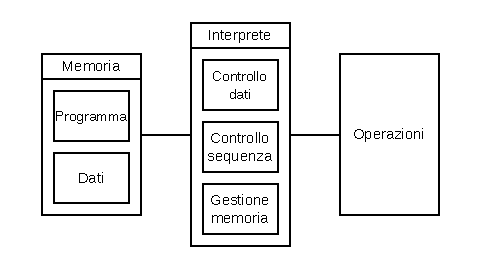
\includegraphics[width=\linewidth]{ma.pdf}}
    \caption{Struttura generale di una m.a.}
\end{figure}

Indipendentemente dal linguaggio ogni interprete ha un flusso di esecuzione e delle operazioni di base comuni:
\begin{itemize}
    \item Operazioni per l'elaborazione dei dati primitivi
    \item Op. e strutture dati per il controllo di sequenza
    \item Op. e s.d. per il trasferimento dei dati
    \item Op. e s.d. per la gestione della memoria\newline
\end{itemize}

\begin{figure}[ht]
    \centering
    \fbox{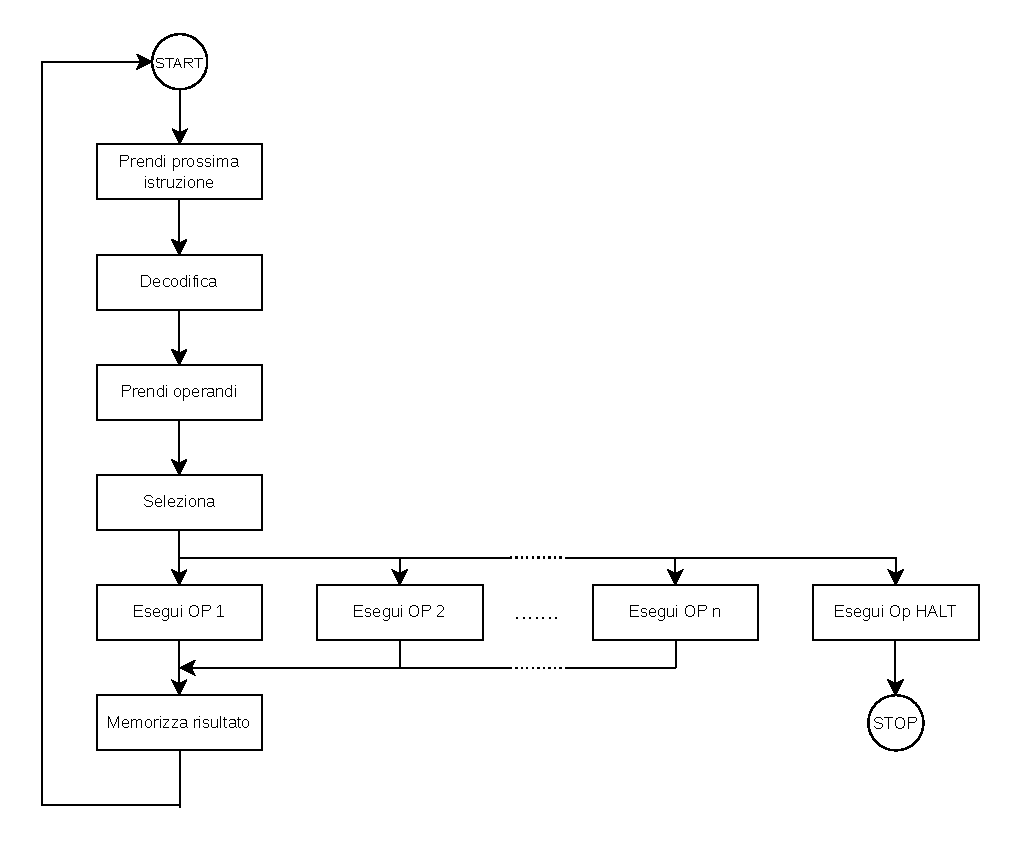
\includegraphics[width=1\linewidth]{flusso.pdf}}
    \caption{Ciclo di esecuzione}
\end{figure}

\newpage

\df Data una m.a. $M_L$. Il linguaggio $L$ ``compreso'' dall'interprete della macchina è detto linguaggio macchina di $M_L$.\newline

Per andare effettivamente a realizzare un m.a. ci sono 3 strade:
\begin{itemize}
    \item Costruirla fisicamente
    \item Simularla tramite un altro linguaggio (la cui m.a. è già implementata)
    \item Combinare entrambi i metodi\newpage
\end{itemize}

Il secondo metodo presenta a sua volta 3 strade:

\begin{figure}[H]
    \centering
    \fbox{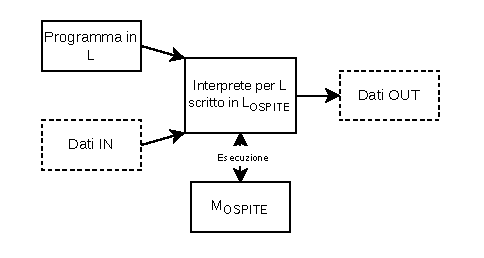
\includegraphics[width=.7\linewidth]{int.pdf}}
    \caption{Interpretazione pura}
\end{figure}


\begin{figure}[H]
    \centering
    \fbox{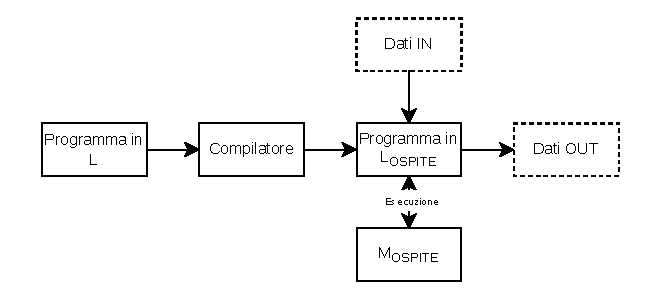
\includegraphics[width=.9\linewidth]{comp.pdf}}
    \caption{Compilazione pura}
\end{figure}

\begin{figure}[H]
    \centering
    \fbox{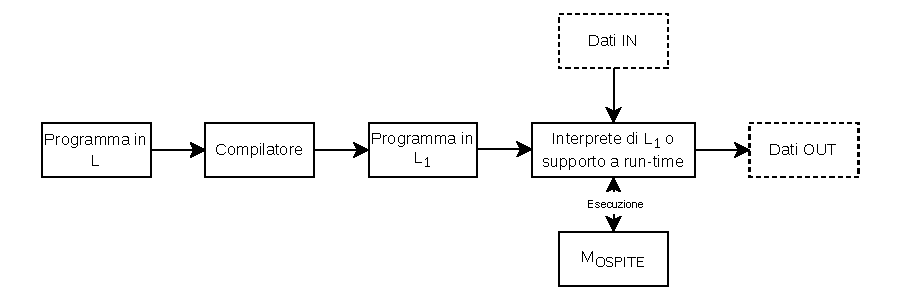
\includegraphics[width=.9\linewidth]{med.pdf}}
    \caption{Via di mezzo (quella più usata nella realtà)}
\end{figure}

In quest'ultimo caso esiste un intero spettro di implementazioni che vanno da quella in cui tutto è simulato a quella in cui tutto è tradotto. La scelta su cosa simulare e cosa tradurre dipende dal linguaggio e dalla macchina ospite, ma in linea di principio i costrutti del linguaggio (da implementare) ``lontani'' dal linguaggio della macchina ospite si simulano e il resto si compila.\newline

L'uso di queste macchine intermedie permette di creare una gerarchia di m.a. simile allo stack ISO/OSI. 

\begin{figure}[ht]
    \centering
    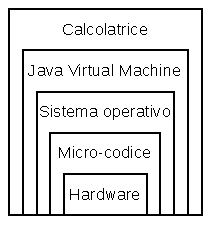
\includegraphics[width=.4\linewidth]{ger.pdf}
    \caption{Esempio di gerarchia}
\end{figure}

\newpage

\section{Descrizione di linguaggi}

Un linguaggio di programmazione può essere descritto su 4 livelli:
\begin{enumerate}
    \item \textbf{Grammatica}

        \begin{enumerate}
            \item \textbf{Lessico}

                Quali sequenze di caratteri formano le parole del linguaggio?
            
            \item \textbf{Sintassi}

                Quali sequenze di parole formano frasi corrette?
            
        \end{enumerate}
    
    \item \textbf{Semantica}

        Che significato ha una certa frase corretta?
    
    \item \textbf{Pragmatica}

        Come si usa una frase corretta in modo sensato?
   
    \item \textbf{Implementazione}
    
        Come va eseguita una frase corretta in modo da rispettarne la semantica?\newline
    
\end{enumerate}

Basandosi su questi concetti si può schematizzare il funzionamento del compilatore:

\begin{figure}[H]
    \centering
    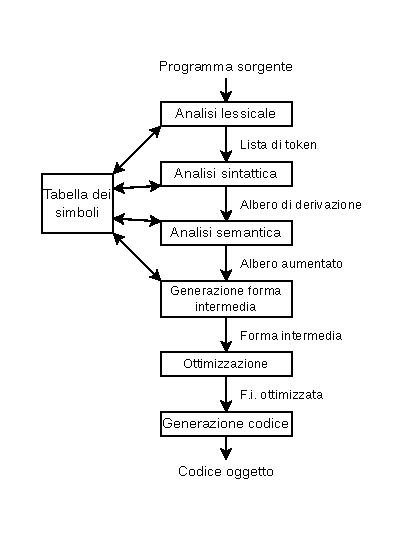
\includegraphics[width=.63\linewidth]{desc_comp.pdf}
\end{figure}

\subsection{Analisi lessicale}

Lo scopo generale dell'analisi lessicale è quello di riconoscere nella stringa di ingresso dei gruppi di caratteri corrispondenti a determinate categorie.

\vspace{5pt}

\begin{table}[ht]
    \centering
    \begin{tabular}{ccc}
        Token & Coppia $\langle$nome,valore$\rangle$ & $\langle IDE,x1\rangle$\\
        Nome & Identifica classe di token & $IDE$\\
        Valore\footnotemark & Identifica specifico token & $x1$\\
        Pattern & Descrizione forma valore & $(x|y)(x|y|0|1)^*$\\
        Lessema & Istanza di un pattern & $x1$\\
    \end{tabular}
\end{table}

\footnotetext{Se nome e valore coincidono spesso quest'ultimo viene omesso.}

Dato che la struttura si esprime sotto-forma di espressione regolare il metodo più naturale per effettuare il riconoscimento è usare un automa. Per esempio nella stringa $if\ (x==0)\ \ printf("zero")$ alcuni token possibili sono:
\begin{itemize}
    \item $\langle CONST-NUM,0\rangle$
    \item $\langle CONST-STR,zero\rangle$
    \item $\langle IDE,x\rangle$
    \item $\langle OP,==\rangle$
    \item $\langle if\rangle$ 
    \item $\langle (\rangle$
    \item $\langle )\rangle$
\end{itemize}

\vspace{5pt}

Dove un possibile automa per le prime 3 categorie è:

\begin{figure}[H]
    \centering
    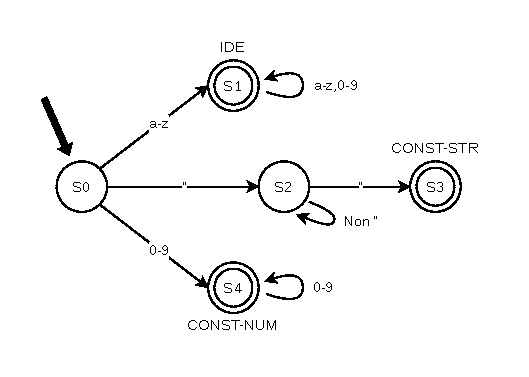
\includegraphics[width=.8\linewidth]{less.pdf}
\end{figure}

\subsection{Analisi sintattica e semantica}

Il passo successivo consiste nel verificare che la sequenza di token data dal punto precedente costituisca una frase formulata correttamente. Per capirlo si definisce un'opportuna grammatica acontestuale e si prova a creare un albero di derivazione, nel caso non sia possibile la frase è mal strutturata.

\begin{figure}[H]
    \centering
    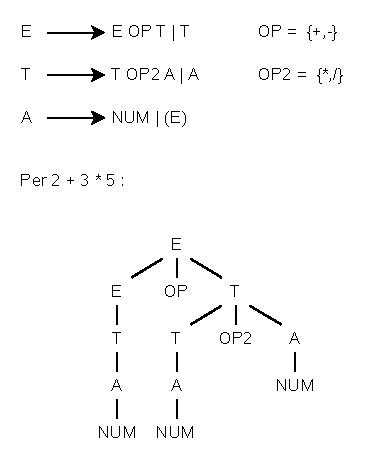
\includegraphics[width=.5\linewidth]{sint.pdf}
    \caption{Esempio di costruzione \textit{top-down}}
    \label{fig:der}
\end{figure}

È anche possibile usare l'approccio \textit{bottom-up}, ossia creare l'albero partendo dalle foglie e andando a ritroso. 

La correttezza di una frase potrebbe però dipendere anche dal contesto in cui essa si trova, per esempio:
\begin{itemize}
    \item In Java una variabile locale di una funzione non si può usare prima che gli venga assegnato un valore;
    \item In Pascal la variabile di controllo usata in un ciclo \textit{for} non si può modificare nello stesso;
\end{itemize}

Questi tipi di vincoli sono detti ``vincoli sintattici contestuali''\footnote{Spesso vengono chiamati ``vincoli di semantica statica'', intesi come vincoli verificabili staticamente sul testo del
programma. Analogamente esistono quelli di ``semantica dinamica'' attinenti al momento di esecuzione del programma.}. L'analisi semantica va a verificare se questi vengano rispettati e facendolo ``aumenta'' man mano l'albero inserendoci informazioni aggiuntive. Facendo una visita dell'albero finale ottenuto si può già ottenere una prima versione del codice (la forma intermedia).

\newpage

\section{Nomi e ambiente}

\df Un nome è una sequenza di caratteri usata per denotare un oggetto\footnote{Un oggetto può essere: una variabile, un parametro, una procedura, una costante, un tipo, ecc...}.\newline

\df L'insieme delle associazioni nomi-oggetti esistenti a run-time in un certo punto del programma ed in un certo momento dell'esecuzione è detto ambiente.\newline

\df Una dichiarazione è un costrutto che permette di introdurre un'associazione nell'ambiente.\newline

\df L'aliasing è la situazione in cui un oggetto è associato a più nomi diversi nello stesso ambiente\footnote{Un esempio è la \textit{union} in C, dove variabili diverse denotano la stessa zona di memoria.}.\newline

\df Un blocco è una regione testuale di un programma delimitata da un inizio ed una fine, si dividono in blocchi di procedure/funzioni e blocchi in-line.\newline

All'entrata/uscita in/da un blocco avviene un cambiamento di ambiente, rispetto al blocco si distinguono:
\begin{itemize}
    \item \textbf{Ambiente locale}
    
        Associazioni dichiarate localmente.
    
    \item \textbf{Ambiente non locale}
    
        Associazioni visibili nel blocco ma non dichiarate localmente.
    
    \item \textbf{Ambiente globale}
    
        Associazioni create all'inizio dell'esecuzione.
    
\end{itemize}

\vspace{5pt}

Per quanto riguarda quello che succede durante il cambio d'ambiente:
\begin{itemize}
    \item \textbf{In entrata}

        \begin{itemize}
            \item Creazione di associazioni locali
            \item Disattivazione di associazioni non locali il cui nome viene ridefinito localmente
        \end{itemize}
    
    \item \textbf{In uscita}

        \begin{itemize}
            \item Distruzione di associazioni locali
            \item Riattivazione di associazioni disattivate\newline
        \end{itemize}
    
\end{itemize}

A livello più generale le operazioni eseguibili su nomi e ambiente sono:
\begin{itemize}
    \item Creazione di un'associazione
    \item Disattivazione di un'associazione
    \item Riattivazione di un'associazione
    \item Distruzione di un'associazione
    \item Riferimento ad un oggetto tramite nome
\end{itemize}

\vspace{3pt}

Invece per gli oggetti:
\begin{itemize}
    \item Creazione\footnote{In alcuni linguaggi la creazione di un oggetto, di un nome e l'associazione tra i 2 è simultanea.}
    \item Distruzione
    \item Accesso
    \item Modifica\newline
\end{itemize}

Sorge però un problema di visibilità nell'ambiente non locale, per esempio nel seguente codice la $x$ usata dentro $p()$ a quale $x$ esterna si riferisce?

\begin{algorithm}
\SetKwBlock{A}{A}{}
\SetKwBlock{B}{B}{}
\SetKwProg{Proc}{procedure}{}

\A{
    $int\ x \gets 0$\;

    \Proc{p()}{
        $x \gets 1$\;
    }

    \B{
        $int\ x$\;
        \texttt{$p$}()\;
    }

    \texttt{write}($x$)\;
}
\end{algorithm}

Per evitare casi di questo tipo va usata una regola di scope (visibilità), ce ne sono 2:
\begin{itemize}
    \item \textbf{Statico}

        Si cerca nel blocco superiore, se non c'è in quello si continua a salire. 
        
        ($x$ di \textbf{A}, alla fine viene stampato 1)
    
    \item \textbf{Dinamico}

        Si usa l'occorrenza più recente da un punto di vista temporale. 
        
        ($x$ di \textbf{B}, alla fine viene stampato 0 perché la $x$ di $B$ sparisce uscendo dal blocco)
    
\end{itemize}

\vspace{2pt}

\section{Gestione della memoria}

\df Un record di attivazione (o frame) è uno spazio in memoria allocato per una procedura o in generale per un blocco.\newline

Una m.a. può gestire la memoria in 3 modi:
\begin{enumerate}
    \item \textbf{Staticamente}

        \begin{minipage}[t]{0.55\linewidth}
        Prima dell'esecuzione il compilatore va a designare un'area di memoria apposita per ogni oggetto. Questo metodo è perfetto per le variabili locali, le costanti e le singole istruzioni del codice oggetto. Nel caso in cui il linguaggio non supporti la ricorsione si può estendere il metodo anche alle procedure salvando in memoria le loro informazioni locali\footnotemark.
        \end{minipage}
        \hfill
        \begin{minipage}[t]{0.4\linewidth}
            \centering
            \begin{tabular}[t]{|c|}
                \hline
                \textbf{Procedura 1} \\
                \hline
                Info di sistema \\
                \hline
                Indirizzo di ritorno \\
                \hline
                Parametri \\
                \hline
                Variabili locali \\
                \hline
                Risultati intermedi \\
                \hline
            \end{tabular}
        \end{minipage}

        \footnotetext{Chiamate diverse alla stessa funzione fanno riferimento alla stessa zona di memoria.}
    
    \item \textbf{Dinamicamente}

        \begin{enumerate}
            \item \textbf{Con pila}

                \begin{minipage}[t]{0.65\linewidth}
                L'ingresso in un blocco comporta l'inserimento di un RdA dentro una pila (poi rimosso all'uscita) che viene collegato a quello immediatamente precedente tramite puntatore.
                \end{minipage}
                \hfill
                \begin{minipage}[t]{0.3\linewidth}
                    \centering
                    \begin{tabular}[t]{|c|c|}
                        \hline
                        \textbf{In-line} & \textbf{Procedura}\\
                        \hline
                         & Puntatore catena statica \\
                        \hline
                        \multicolumn{2}{|c|}{Puntatore catena dinamica} \\
                        \hline
                        \multicolumn{2}{|c|}{Variabili locali}\\
                        \hline
                        \multicolumn{2}{|c|}{Risultati intermedi} \\
                        \hline
                         & Parametri \\
                        \hline
                         & Indirizzo di ritorno \\
                        \hline
                         & Indirizzo del risultato \\
                        \hline
                    \end{tabular}
                \end{minipage}
            
            \item \textbf{Con heap}

                Se il linguaggio prevede comandi per l'allocazione esplicita di memoria si definisce una zona specifica dove è possibile riservare blocchi di dimensioni fisse/variabili.
            
        \end{enumerate}

\newpage
    
\end{enumerate}

\section{Meccanismi di controllo}

\df  Un'espressione è un'entità sintattica la cui valutazione produce un valore oppure non termina. Generalmente è composta da una singola entità o da un operatore applicato a degli operandi.\newline

Per il secondo caso esistono diversi metodi di rappresentazione:
\begin{itemize}
    \item \textbf{Notazione infissa}

        $$(a+b)*(c+d)$$
    
    \item \textbf{Notazione prefissa}\footnote{Anche detta notazione polacca.}

        $$*(+(a\ b)+(c\ d))$$
    
    \item \textbf{Notazione postfissa}\footnote{Anche detta notazione polacca inversa.}

        $$((a\ b)+(c\ d)+)*$$
    
\end{itemize}

\vspace{2pt}

\noindent(Nelle ultime 2 si possono omettere le parentesi se si conosce l'arietà delle operazioni)\newline

Cambiando la notazione cambia anche il metodo di valutazione, rispettivamente:
\begin{itemize}
    \item Bisogna definire delle regole di precedenza, altrimenti serve un uso massiccio di parentesi;
    
    \item Scansione da sinistra a destra ed uso di una pila;

    \item Come il precedente.
    
\end{itemize}

Ogni notazione si può ottenere con un tipo di visita diversa dell'albero di derivazione (considerando solo i simboli terminali), per esempio nella figura \ref{fig:der}:

\vspace{4pt}

\begin{minipage}[t]{0.65\linewidth}
\begin{itemize}
    \item \textbf{In ordine}\footnotemark

        NUM OP NUM OP2 NUM$\rightarrow2 + 3 * 5$

    \item \textbf{Pre-ordine}\footnotemark

        OP NUM OP2 NUM NUM$\rightarrow+\ 2\ *\ 3\ 5$
    
    \item \textbf{Post-ordine}\footnotemark

        NUM NUM NUM OP2 OP$\rightarrow2\ 3\ 5\ *\ +$
    
\end{itemize}
\end{minipage}
\hfill
\begin{minipage}[t]{0.25\linewidth}
    \begin{figure}[H]
        \centering
        \fbox{
        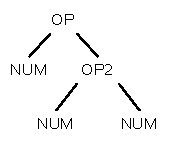
\includegraphics[width=.7\linewidth]{sint2.pdf}
        }
    \end{figure}
\end{minipage}

\footnotetext[9]{Sx, radice, dx.}
\footnotetext[10]{Radice, sx, dx.}
\footnotetext{Sx, dx, radice.}

\vspace{4pt}

\newpage

\df Un effetto collaterale è un'azione che
influenza i risultati di una computazione senza restituire esplicitamente un valore.\newline

\df Un comando è una entità sintattica la cui valutazione non necessariamente restituisce un valore, ma può avere un effetto collaterale.\newline

\df Una variabile modificabile è una locazione di memoria (con nome) contenente dei valori che possono cambiare nel tempo.\newline

Alcuni comandi:
\begin{itemize}
    \item Assegnamento
    \item \textbf{Controllo di sequenza}
        \begin{itemize}
            \item \texttt{;}
            \item \texttt{Begin}$\ldots$\texttt{End}
            \item \texttt{GOTO}
            \item \texttt{Continue}
            \item \texttt{Break}
            \item \texttt{Return}
        \end{itemize}
    \item \textbf{Condizionali}
        \begin{itemize}
            \item \texttt{If} (e sue varianti)
            \item \texttt{Switch}$\ldots$\texttt{Case}$\ldots$\texttt{Default}
        \end{itemize}
    \item \textbf{Iterativi}
        \begin{itemize}
            \item Indeterminati
                \begin{itemize}
                    \item \texttt{While}
                    \item \texttt{Do}$\ldots$\texttt{While}
                    \item \texttt{Repeat}
                    \item \texttt{Until}
                \end{itemize}
            \item Determinati
                \begin{itemize}
                    \item \texttt{For}
                    \item \texttt{For-each}
                \end{itemize}
        \end{itemize}
\end{itemize}

\newpage

\section{Funzioni}

\df Una funzione è una porzione di codice identificata da un nome\footnote{Il nome della funzione appartiene all'ambiente non locale}, dotata di ambiente locale proprio e capace di scambiare informazioni col resto del codice mediante parametri\footnote{Si distinguono quelli che appaiono nella definizione (\textit{formali}) e quelli che appaiono nella chiamata (\textit{attuali}).}, valore di ritorno e ambiente non locale. \newline

Esistono diversi metodi di funzionamento dei parametri:
\begin{itemize}
    \item \textbf{Per valore}

        I parametri formali copiano i valori dei parametri attuali.
    
    \item \textbf{Per riferimento}

        I parametri formali diventano degli alias dei parametri attuali.      
    
    \item \textbf{Per costante}

        Come il precedente ma \textit{read-only}.
    
    \item \textbf{Per risultato}

        Come quello per valore ma in uscita.
    
    \item \textbf{Per valore-risultato}

        Valore + risultato.
    
    \item \textbf{Per nome}

        Le occorrenze dei parametri formali vengono sostituite con quelli attuali, per esempio in:

        \begin{algorithm}
            \SetKwBlock{A}{}{}
            \SetKwBlock{B}{foo(name int $y$)}{}
            \A{
                $int\ x \gets 2$\;
            
            
                \B{
                    \texttt{return} $y+y$\;
                }
            
                $a\gets$\texttt{foo}($x++$)\;
            }
        \end{algorithm}

        $y+y$ diventa $(x++)+(x++)$ dove $x++$ viene valutato ad ogni occorrenza, quindi:
        \begin{enumerate}
            \item Il primo operando è 2
            \item $x$ diventa 3
            \item Il secondo operando è 3
            \item $x$ diventa 4
            \item $a$ è 5
        \end{enumerate}
    
\end{itemize}

\vspace{3pt}

\end{document}
